\chapter{Úvod}\label{chap:intro}

\chapter{Motivácia}\label{chap:motivation}

\chapter{Východiská}\label{chap:intro}
V tejto kapitole je cieľom poskytnúť prehľad základným pojmom a postupov pri tvorbe verifikačného 
nástroja pre programovaní jazyk UNITY.

\section{UNITY}

UNITY vychádza z knihy Parallel Program Design - A Foundation, v ktorej bol UNITY popísaný a 
navrhnutý autormi K. Mali Chandy a Jayadev Misra z Univerzity of Texax. Je to teoretický jazyk, 
ktorý sa zameriava na to \textbf{čo}, namiesto toho \textbf{kde}, \textbf{kedy} alebo \textbf{ako}. 
Jazyk neobsahuje žiadnu metódu \textbf{riadenia toku} a príkazy programu prebiehajú 
\textbf{nedeterministickým spôsobom} \textbf{synchrónne a asynchrónne}, kým sa \textbf{priradenia} nedostanú do konečného \textbf{stavu}.
To umožňuje, aby programy bežali na neurčito, ako napríklad autopilot alebo elektráreň, ktoré by normálne skončili.

\section{Vlastnosti UNITY}

\begin{itemize}
	\item Nedeterminizmus
	\item Absencia toku riadenia (control-flow)
	\item Synchrónnosť a asynchrónnosť
	\item Stavy a priradenia
\end{itemize}


\subsection{Nedeterminizmus}
Je algoritmus, ktorý si môže vybrať z viacerých možností, ktoré má k dispozicií. Nedeterministický algoritmus 
môže pri rovnakých vstupoch dávať rozdielné výsledky. Konkrétne v UNITY to znamená, že jednotilvé príkazy a priradenia 
sa budú vykonávať v rozdielnom poradí, čo môže mať za dôsledok rozdielné výsledky programu.

\subsection{Absencia riadenia toku (control-flow)}
Takýto tok nám zabezpečí paralelné vykonávanie programu. V prvotných programovacích jazykoch sa control-flow používal
na postupné riadenie procesov. V prípade UNITY je takéto riadenie procesov zabezpečené paralelizmom.

\subsection{Synchrónnosť a asynchrónnosť}
Ako všetky programovacie jazyky, ktoré sú založené na paralelizme aj UNITY využíva synchronné a asynchrónne operácie. 

\subsection{Stavy a priradenia}
Stavy a priradia sú základom UNITY programu. Konkrétne tento prechodový systém pozostáva z počiatočného stavu a transformácií, 
ktoré sú reprezentované premennými a priradeniami. Do výsledného stavu sa program dostane pomocou niekoľkých priradení, pri ktorých 
premenné nadobúdajú výsledné hodnoty.

\section{Telo programu}

UNITY obsahuje štyri základné sekcie: decleráciu premmenných, množinu skratiek, 
počiatočné hodnoty premenných a množinu priraďovacích príkazov. 
V tele programu sa tieto sekcie vyskytujú pod názvamy declare, always, 
initially, assign. Telo programu obsahuje aj program-name, názov programu, 
ktorý môžeme vynechať, v tom prípade z tela programu vynechávame aj sekciu program-name. 
UNITY program má nasledujúcu formu:

\begin{lstlisting}
Program 				program-name
	declare 			declare-section
	always	 		always-section
	initially 		initially-section
	assign 			assign-section
end
\end{lstlisting}


\subsection{Declare-section}

Táto sekcia obsahuje dekleráciu premenných použité v programe a ich súvisiace typy. 
V nasledujúcej ukážke môžete vidieť dekleráciu premenných x a y typu integer. 
Syntax je podobná ako v programovacom jazyku PASCAL. Medzi základné typy patria:
\begin{itemize}
	\item Integer
	\item Boolean
\end{itemize}

\vspace{5mm}

Príklad deklerácie:
\begin{lstlisting}
declare 
	x, y : integer
	b : boolean
\end{lstlisting}

\vspace{5mm}

Taktiež sa využívajú n-rozmerné polia v nasledujúcom tvare:
\begin{lstlisting} d
declare 
	p: Array[a1, a2, ..., an] of integer
\end{lstlisting}

\subsection{Always-section}

Sekcia always definuje skratky, ktoré slúžia na stručné spísanie programu. 
Konkrétnejšie to sú premenné, ktoré definujú funkcie alebo podmienky. 
Takéto premenné sú známe ako transparentné premenné. 
Transparentné premenné poskytujú vhodný spôsob skrátenia výrazov, ktoré sa často vyskytujú v programe. 
Táto sekcia nie je nevyhnutná v tele programu UNITY. Transparentné premenné môžeme definovať následovne pomocou ||:

\begin{lstlisting}
always
		decx = x > y
	||
		decy = y > z
\end{lstlisting}

Tieto premenné je možné zapísať aj jednoriadkovo bez použitia spojovníka:

\begin{lstlisting}
always
	decx, decy = z > y, y > z
\end{lstlisting}

\subsection{Initially-section}

Initially sekcia je súbor rovníc, ktoré definujú počiatočné hodnoty pre niektoré programové premenné. 
Premenné, ktoré nie sú inicializované majú ľubovoľné počiatočné hodnoty. Premenné x a y môže byť definované:

\begin{lstlisting}
initially
		x = X
	||
		y = Y
\end{lstlisting}

alebo takto:

\begin{lstlisting}
initially
	x, y = X, Y
\end{lstlisting}
\subsection{Assign-section}
Táto sekcia je konečná a neprázdna množina, ktorá sa skladá z konečných príkazov, tie sú oddelené znakom []. 
Znak [] predstavuje nedeterminizmus. Príkazy sa skladájú z konečných priradení, tie sú oddelené znakom ||.
Tento znak predstavuje paralelizmus. Príklady:
\begin{lstlisting}
	assign
		x, y := 1, 2 
	[]	x, y := y, x if x > y	
\end{lstlisting}

V týchto príkladoch môžeme vidieť dve rôzne priradenia, podmienené a nepodmienené. 
Podmienené priradenie obsahuje podmienku \textit{if x > y}, ktorá musí byť splnená ak dané priradenie má byť vykonané.
V tomto konkrétnom príklade ak je \textit{x} väčšie ako \textit{y} tak \textit{x} sa rovná \textit{y} a \textit{y} sa rovná \textit{x}.
Nepodmienené priradenie je teda jednoduché priradenie, v ktorom nie je žiadna podmienka a priradenie sa vykoná.
Ďaľšie priradenia, ktoré sa môžu v assign sekcii vyskytnúť sú \textbf{kvantifikované priradenia} a \textbf{kvantifikované výrazy}.

\subsubsection{Kvantifikované priradenia}

Kvantifikované priradenia slúžia na zapísannie konečnej množiny priradení. Príklad:
\begin{lstlisting}
	assign
		<|| i, j : 1 =< i, j =< 10 :: A[i, j] := 0 >
	resp.
		<[] i, j : 1 =< i, j =< 10 :: A[i, j] := 0 >
\end{lstlisting}
Z tohto príkladu môžeme vidieť, že sa jedná o dvojtý for cyklus, ktorý prechádza dvajrozmerné pole A. 
Časť \textit{i, j} nám hovorí o vytvorení lokálnych premenných, ktoré sa kontrolujú booleovskou podmienkou \textit{1 =< i, j =< 10}.
Ak je podmienka splnená vykoná sa daný príkaz \textit{A[i, j] := 0}. 
Znak || nám hovorí, že sa ma príkaz bude vykonávať paralelne a znak [], že sa bude vykonávať nedeterministicky.
Od takéhoto priradenia požadujeme aby sa nestal zacykleným resp. bol konečným 
a v prípade, že bude obsahovať vnorené kvantifikované priradenie musí byť konečné.

\subsubsection{Kvantifikované výrazy}

\vspace{5mm}
Kvantifikované výrazy obsahujú binárnu operáciu. Napríklad tento výraz
\begin{lstlisting}
	assign
		<max i, j, k : 1 =< i, j, k =< N :: A[i, j, k] >
\end{lstlisting}
nám vráti maximálny prvok z trojrozmenrného poľa A. Ak nám daný výraz vráti prázdnu množinu tak 
nadobúda hodnotu, ktorá patrí neutrálnemu prvku operácie. Binárne operácie a jej neutrálny prvok sú:

\begin{center}
\begin{tabular}{|c|c|}
\hline
Binárna operácia & Neutrálny prvok \\
\hline
min              & \infinity       \\
\hline
max              & -\infinity      \\
\hline
+                & 0               \\
\hline
*                & 1               \\
\hline
$\land$          & true            \\
\hline
$\vee$           & false           \\
\hline
$\equiv$         & true            \\
\hline
\end{tabular}
\end{center}

\subsection{Vykonanie programu UNITY}
Na začiatku programu je najdôležitejšia declare sekcia, kde sa deklerujú všetky premenné. 
Následne na to program postupuje do initial sekcie, tú sa deklerované premenné inicializujú, tie ktoré 
inicializované nie sú nadobúdajú náhodnú hodnotu. Ak je zadefinovaná always sekcia vykoná sa aj tá, 
priradia sa všetky transparentné premenné. V poslednom kroku program pokračuje do assing sekcie.
Spustí sa nekonečný cyklus nedeterministického vyberania príkazov, ktoré obsahujú priradenia 
vykonávajúce sa paralelne. Každý z týchto krokov v assing sekcii sa vykonáva nekonečne veľa krát.

\subsubsection{Pevný bod}

Počas vykonávania programu môže nastať situácia vytvorenia tzv. \textbf{pevného bodu}, 
alebo \textbf{Fixed Point}. Tento bod predstavuje stav programu, kedy sa aktuálny stav programu
už nikdy nezmení. V našom prípade to bude znamenať ukončenie programu.


\begin{lstlisting}
Program 				GCD
	declare 			x, y : integer
	initially	 	x, y = X, Y
	assign 			x := x - y if x > y
				||		y := y - z if y > x
end
\end{lstlisting}

\section{Interpreter}
Interpreter je počítačový program, ktorý interpretuje iný program napísaný 
v nejakom programovacom jazyku. Interpretre môžu program interpretovať riadok 
po riadku alebo preložia program do nejakého medzikódu a tento medzikód potom vykonávajú. 
Ak je v programe syntaktická chyba, prvý druh interpretra vykoná program po túto syntaktickú 
chybu a zahlási chybu na príslušnom riadku, druhý druh interpretra program nezačne vykonávať a
počas prekladu do medzikódu zahlási chybu.

Programy vykonávané interpretrom bežia väčšinou pomalšie, ako kompilované programy.

Interpreter môže byť vo všeobecnosti interpretátorom ľubovoľného formalizovaného jazyka, 
napríklad interpreter matematických výrazov. Známe interpretre: PHP, Python MATLAB, Perl...

\begin{figure}[h]
\centerline{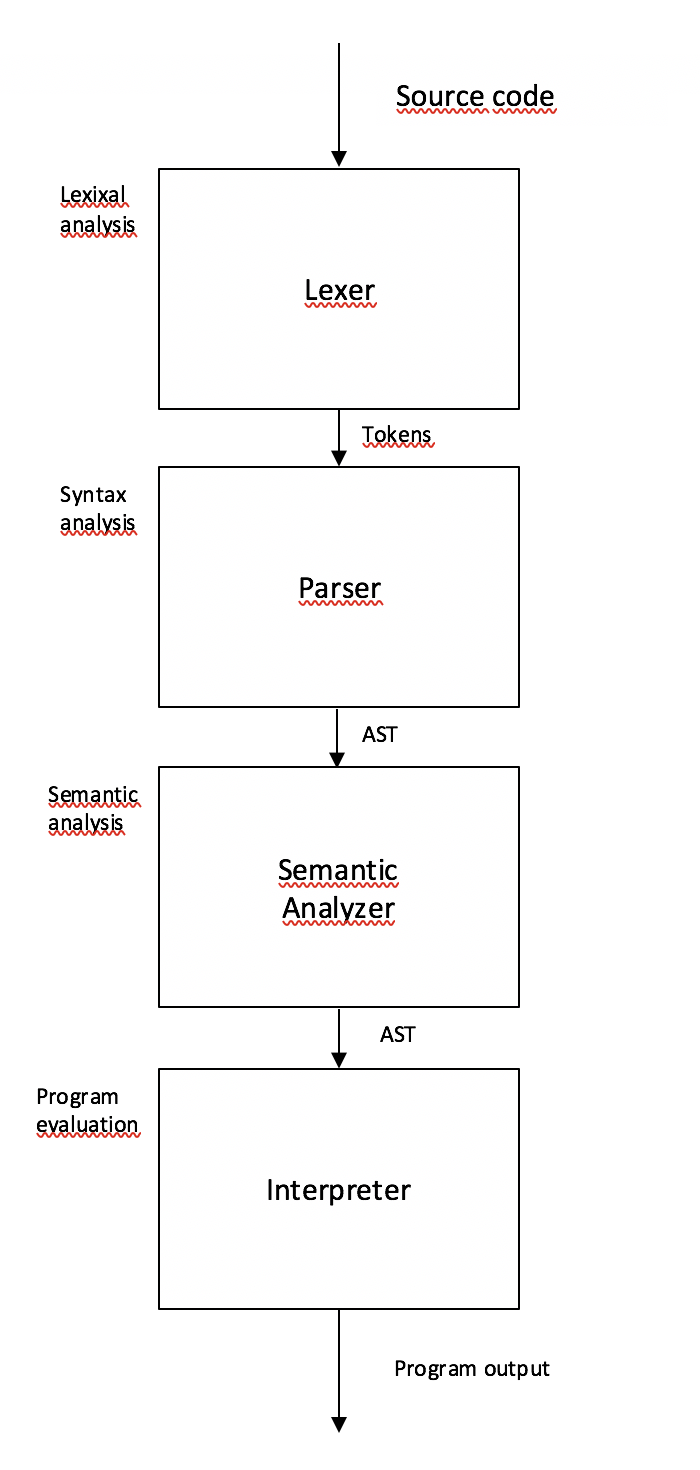
\includegraphics[width=0.4\textwidth]{images/intepreter}}
\caption[intepreter]{Štruktúra intepretra}
\label{obr:intepreter}
\end{figure}

\subsection{Štruktúra interpretra}
Interpreter sa skladá z troch častí: front-end, middle-end a back-end.

\begin{enumerate}
	\item Front-end (Predná časť) - overuje syntax a sémantiku špecifickú pre daný zdrojový kód. 
	Pokiaľ je program na vstupe syntakticky nesprávny, obsahuje syntaktickú chybu, 
	interpreter by mal vhodným spôsobom na to reagovať. 
	Predná časť spravidla zahŕňa lexikálnu analýzu, syntaktickú analýzu a sémantickú analýzu.
	Výstupom prác prednej časti interpretru býva program v intermediárnom kóde, 
	ktorý je poskytovaný na spracovanie nasledujúcim častiam intrepretru.

	\item Middle-end (Stredná časť) - vykonáva optimalizácie nad intermediárnym kódom. 
	Tieto optimalizácie sú nezávislé na architektúre cieľového počítača. 
	Príkladom optimalizácií v strednej časti prekladu je odstraňovanie zbytočných 
	alebo nedosiahnuteľných častí kódu, či optimalizácia cyklov. Výstupom tejto časti intrepretra 
	je "optimalizovaný" intermediárny kód, ktorý je následne používaný zadnou časťou intrepretra.

	\item Back-end (Zadná časť) -  môže vykonávať dodatočnú analýzu a optimalizácie, 
	ktoré sú špecifické pre cieľový počítač. V každom prípade je však jej hlavnou úlohou 
	generovanie cieľového kódu.
\end{enumerate}

\subsection{Lexikálna analýza, syntaktická analýza a sémantická analýza}

\subsubsection{Lexikálna analýza}
Lexikálna analýza je činnosť, ktorú má na starosť tzv. lexikálny analyzátor - 
je súčasťou prekladača. Lexikálny analyzátor rozdelí vstupnú postupnosť znakov na \textbf{lexémy}. 
Tieto lexémy sú reprezentované ve forme tokenov (symbolov), tie sú poskytnuté 
ku spracovaniu syntaktickému analyzátoru.

\textbf{Lexémy} sú základné symboly programovacieho jazyka, patria sem identifikátory,
kľúčové slová, konštanty rôznych typov, operátory.

\subsubsection{Syntaktická analýza}
Syntaktická analýza sa v informatike nazývá proces analýzy postupnosti 
formálnych prvkov s cieľom určiť ich gramatickú štruktúru voči predom danej formálnej gramatike.
Program, ktorý vykonává tuto úlohu, se nazývá syntaktický analyzátor (parser) - 
vstupný text transformuje na určité datové struktury, syntaktický strom, 
ktorý zachováva hierarchické usporiadanie vstupných symbolov, ktoré sú vhodné pre daľšie spracovanie.

\subsubsection{Sémantická analýza}
Sémantická analýza postupne prechádza symboly či skupiny symbolov získané 
zo syntaktickej analýzy a priraďuje sa im význam. Pokiaľ napríklad skupina symbolov
predstavuje použitie konkrétnej premennej, tak analyzátor zisťuje či je premenná už 
deklarována a či je správne použita vzhľadom k jej datovému typu.

\subsection{Syntaktický strom}
Abstraktný syntaktický strom je v informatike stromovou reprezentaciou 
abstraktnej syntaktickej štruktúry zdrojového kódu 
napísaného v programovacom jazyku. 
Abstraktný syntaktický strom se využívá primárne na preklad a optimalizaciu kódu.

\subsubsection{Štruktúra syntaktického stromu}

\begin{itemize}
	\item vnútorné uzly stormu sú operátory

	\item listy stromu sú jeho operandy

	\item každá časť podstromu je samostatnou logickou jednotkou
\end{itemize}

Nasledujúci obrázok vychýdza z daného kódu
\begin{lstlisting}
	while b != 0:
		if a > b:
			a = a - b
		else:
			b = b - a
	return a
\end{lstlisting}

\begin{figure}[ht]
\centerline{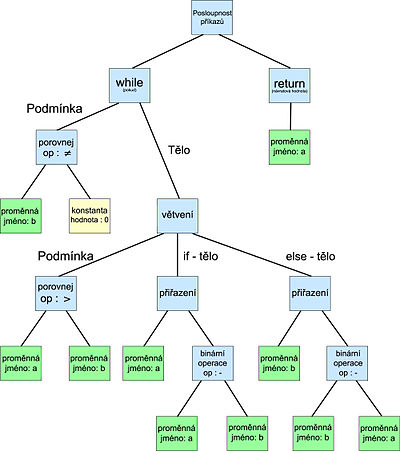
\includegraphics[width=0.5\textwidth]{images/syntakticky_strom}}
\caption[Syntaktický strom]{Syntaktický strom}
\label{obr:tree}
\end{figure}

\subsection{Model checking}
Overovanie modelov alebo model checking je automatizovaná metóda formálnej verifikácie 
paralelného systému s konečným počtom stavov. Kontroluje sa, či zadaný model vyhovuje špecifikácii. 
Model sa zadáva ako systém prechodov stavov, kde vrcholy sú stavy, a postupnosť prechodov predstavuje
vykonávanie správania sa modelu. Špecifikácia systému sa zadáva formulami temporálnej logiky. 
Výsledkom verifikácie je odpoveď na otázku, či model spĺňa špecifikáciu cite \cite{br4}.

\textbf{Temporálna logika}  je odvetvie logiky, ktoré skúma logickú štruktúru výrokov 
o čase s ktorými klasická výroková alebo predikátová logika nedokážu plnohodnotne narábať.

\subsubsection{Výhody}

\begin{itemize}
	\item Žiadne dôkazy
	\item Rýchlosť
	\item Kontra príklady
	\item Žiadne problémy s čiastočnými špecifikáciami
	\item Logika môže vyjadriť veľa súbežných vlastností
\end{itemize}

\subsubsection{Nevýhody}

\begin{itemize}
	\item Príliš veľa procesov
	\item Dátové cesty
\end{itemize}

\subsection{LTSmin}
LTSmin (model checker) začal ako všeobecná sada nástrojov na manipuláciu s označenými prechodovými systémami. 
Medzitým bola sada nástrojov rozšírená na plný overovací model, 
pri zachovaní jeho jazykovo nezávislých charakteristík.

Na získanie svojho vstupu LTSmin spája značný počet existujúcich overovacích 
nástrojov: muCRL , mCRL2 , DiVinE , SPIN (SpinS), UPPAAL (opaal), SCOOP , PNML , ProB a CADP.

LTSmin má modulárnu architektúru, ktorá umožňuje prepojenie viacerých front-end modelovacích 
jazykov s rôznymi analytickými algoritmami prostredníctvom spoločného rozhrania.
Poskytuje symbolické aj explicitné algoritmy analýzy viacerých jazykov, 
ktoré umožňujú viaceré spôsoby riešenia problémov pri konflikte.
Toto prepojovacie rozhranie sa nazýva Partitioned Next-State Interface (PINS), 
ktorého základom je definícia stavového vektora, počiatočný stav, 
funkcia NextState a funkcie označovania.

\begin{figure}[ht]
\centerline{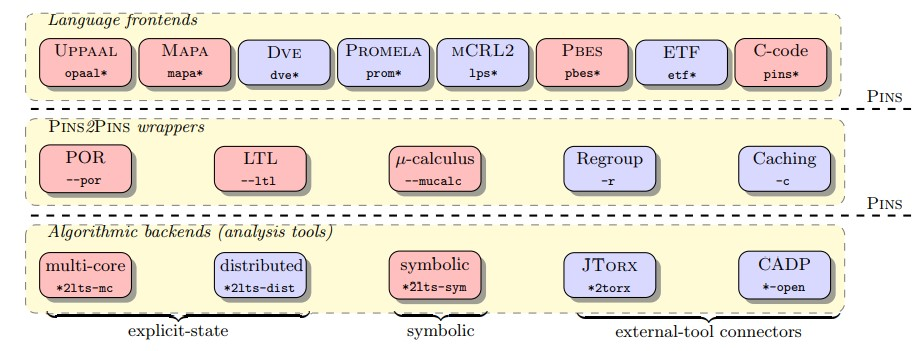
\includegraphics[width=1\textwidth]{images/ltsmin}}
\caption[PINS architektúra]{PINS architektúra}
\label{obr:pins}
\end{figure}

\subsubsection{Back-ends}
LTSmin ponúka rôzne analytické algoritmy zahŕňajúce tri algoritmické backendy:

\begin{itemize}
	\item Distribuované inštancie
	\item Viacjadrový model
	\item Symbolická kontrola modelu
\end{itemize}

\subsubsection{Front-ends}
LTSmin už spája značný počet existujúcich overovacích nástrojov ako jazykových modulov, 
čo umožňuje používať ich modelové formalizmy:

\begin{itemize}
	\item muCRL
	\item mCRL2
	\item DiVinE
	\item SpinS
	\item UPPAAL
	\item SCOOP
	\item PNML
	\item ProB
	\item CADP
\end{itemize}

\subsubsection{PINS2PINS}
Rozhranie PINS čisto rozdeľuje naše kontrolné nástroje do dvoch nezávislých častí: 
\begin{itemize}
	\item jazykové moduly
	\item algoritmy kontroly modelov
\end{itemize}
Umožňuje však aj vytvorenie modulov PINS2PINS, 
ktoré sa nachádzajú medzi jazykovým modulom a algoritmom.
Tieto moduly PINS2PINS môžu využívať všetky algoritmické backendy a 
môžu byť zapnuté a vypnuté na požiadanie:

\begin{itemize}
	\item Transition caching do vyrovnávacej pamäte zvyšuje pomalé jazykové moduly
	\item Regrouping urýchľuje symbolické algoritmy pomocou optimalizácie závislostí
	\item Partial-order znižuje stavový priestor tým, že klesne irelevantné prechody
\end{itemize}

\begin{figure}[ht]
\centerline{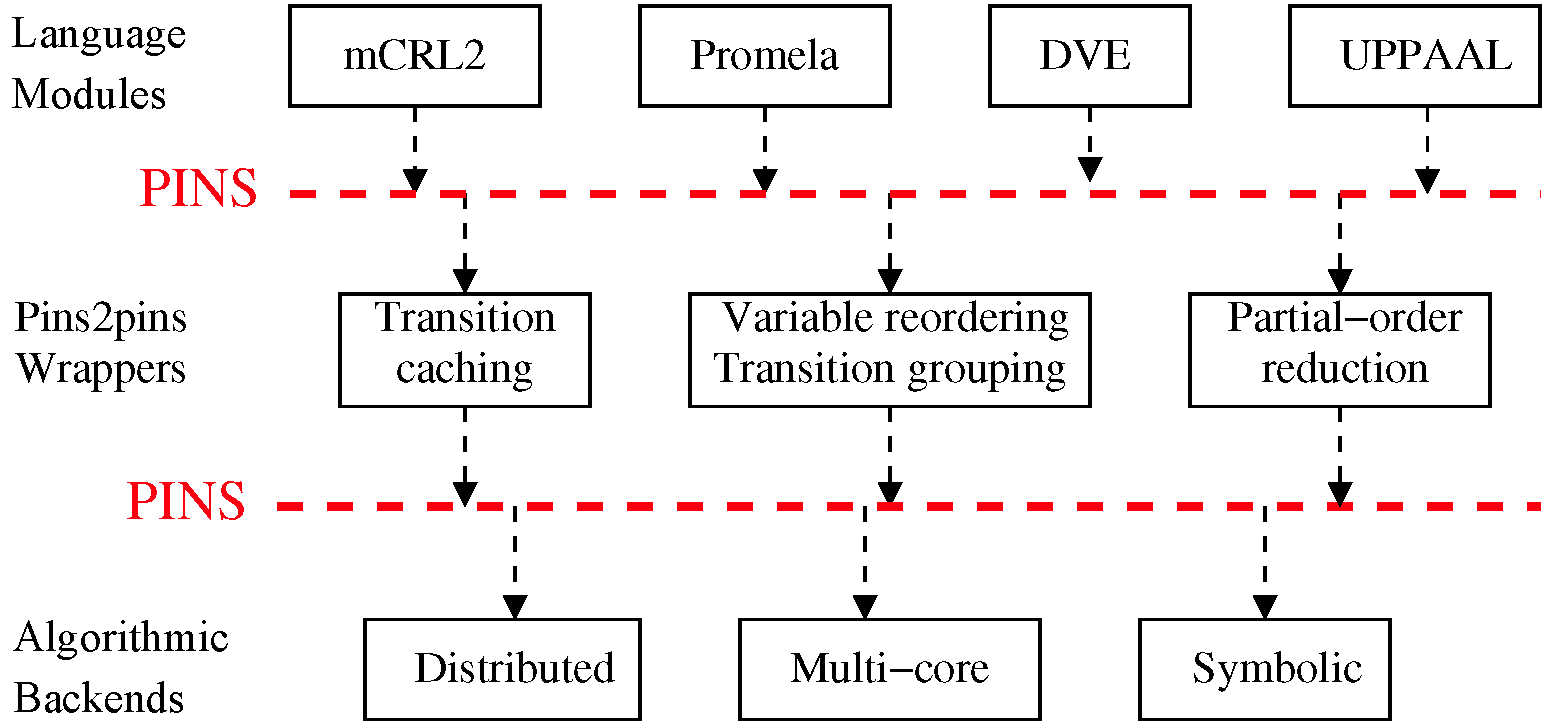
\includegraphics[width=0.7\textwidth]{images/pins2pins}}
\caption[PINS2PINS]{PINS2PINS}
\label{obr:pins2pins}
\end{figure}